\documentclass[12pt]{article}
\usepackage{coursenote}

\renewcommand\vec[1]{\ensuremath{\mathbf{#1}}}

\begin{document}
\title{STAT 401 Chapter 10.2--10.4}
\maketitle

\section{Identifying outlying $X$ observations:\\ leverage $h_{ii}$}

\subsection{What can go wrong?}

With a one-predictor model, we can demonstrate
three note-worthy problems of a certain data point $(x_i, y_i)$:

\begin{enumerate}
\item Outlying in terms of $X$
    \begin{enumerate}
        \item $y_i$ is away from the ``expected'' $Y$ at this $x_i$
            as is indicated by the trend suggested by the other data points.
        \item $(x_i, y_i)$ is ``in the trend'' but is far from other data
            points.
    \end{enumerate}
\item Within range in terms of $X$
    \begin{itemize}
        \item but $Y$ is ``out of trend''
    \end{itemize}
\end{enumerate}

If there are two predictors, on a $X_1$-$X_2$ scatter plot
it is easy to see whether a data point is outlying in terms of $X$,
but it is harder to check $Y$ (a 3-D plot would be needed).

With three or more predictors,
the above are still the problems to check for,
but it is not easy to do by graphics.
Effective, easy-to-interpret numerical measures are needed.
The secret is in the ``hat'' matrix.

\subsection{``Leverage'' value in terms of $X$}

The outlying-ness of $X$ of the $i$th observation
is indicated by
the $i$th diagonal element of $\mat{H}$, $h_{ii}$,
called \emph{leverage}.
Recall $\mat{H} = \mat{X}\bigl(\mat{X}^T\mat{X}\bigr)^{-1}\mat{X}^T$.
Its $i$th diagonal element is
\[
h_{ii} = \vec{x}_i' (\mat{X}'\mat{X})^{-1} \vec{x}_i
\]
where $\vec{x}_i$ (a column vector)
is the transpose of the $i$th row of $\mat{X}$.
Note: $\vec{x}_i$ has a leading 1 if the model contains intercept.

Note: $h_{ii}$ indicates the ``outlying-ness'' in terms of $X$.
It is natural that this measure does not involve $Y$.
This indicator can be examined even before $Y$ is available.

% \remark
% $\vec{x}'\mat{A}\vec{x}$ is a common pattern of measures of distance.
% For example,
% distance from $\vec{0}$ can be measured by
% $\vec{x}'\vec{x} = \vec{x}' \mat{I} \vec{x}$.
% The matrix $\mat{A}$ has to do with whether different dimensions of
% $\vec{x}$ have un-equal weights and whether they ``interact''
% (for the purpose of distance).
% This matrix is usually related to the covariance matrix of the
% components of $\vec{x}$.

\emph{Properties of $h_{ii}$}:
\[
0 \le h_{ii} \le 1,\quad
\sum_{i=1}^n h_{ii} = p
\]
where
$n$ is sample size and
$p$ is df of the model, i.e.\@ number of $\beta$'s and
number of rows (or columns) in the design matrix $\mat{X}$
and the hat matrix $\mat{H}$.

\example
Figure 10.6, page 398.

\example
Figure 10.7, page 399.

\subsection{Interpretation}

\begin{enumerate}
\item
$h_{ii}$ somehow measures the distance of
$\vec{x}_i$
from the center of all the $X$ vectors (one vector for each case,
or ``observation'', or ``data point'').

\item
A large $h_{ii}$ implies large \emph{leverage on
model estimation}.

We don't want any observation to have much larger leverage than others.
Indeed, in experimental studies,
one strives to lay out $X$ (before proceed to spend money and time
measuring $Y$) such that no case has exceptionally large leverage
on the model estimation.

\item
How large is too large?
The average leverage is
\[
\overline{h} = \frac{\sum h_{ii}}{n} = \frac{p}{n}
\]
\emph{Rule of thumb}:
when $n \gg p$,
a $h_{ii}$ that is $> 2\overline{h}$ or $> 0.5$ is suspicious.

\item
Although a high-leverage point is influential on the model estimation,
its $Y$ is not necessarily ``out of trend'' in a particular dataset.
However,
imagine its $Y$ observation is indeed in disagreement with the trend
suggested by the other cases.
Then the strong influence on the model estimation exerted by this data
point will show: it will ``pull'' the regression line towards itself.

Also see comment~1 on the top of page~399.
(The comment is not totally accurate. Take it informally.)

\item
Although it's convenient to remember $h_{ii}$
with reference to the hat matrix $\mat{H}$,
this measure really revolves around $\bigl(\mat{X}^T\mat{X}\bigr)^{-1}$,
not $\mat{H}$.
Here's how we can apply the idea to a $\vec{x}$ that is not in the
set of model-building points.

Suppose we apply the fitted model to a new predictor vector
$\vec{x}_*$.
Is the model applicable at this $\vec{x}_*$?
Check whether
\[
h_* = \vec{x}_*' (\mat{X}'\mat{X})^{-1} \vec{x}_*
\]
is notably larger than the leverages of the available data points.
The above empirical rules may be used.
If $h_*$ is too big,
it suggests we are \emph{extrapolating} the model too much.
\end{enumerate}

\section{Identifying outlying $Y$ observations:\\ residuals}

Using $h_{ii}$ we can basically identify the data points
that are outlying in terms of $X$.
Remaining data points that are problematic are those whose
$X$ is within the range of the other $X$'s but whose $Y$ is
``out of trend''.

We identify problematic $Y$ through residuals.
Obviously, a large residual is bad.
However, the ``raw residuals'' have limitations.
Consider data points close to the ``center'' of the ``data cloud''
and those on the outskirts.
A fitted model fits the central part best, meaning
$E(\hat{Y})$ in the central part has small variance
than on the outskirts.
In other words,
the residuals in the central part have small variance than on the
outskirts.
Whether a residual is ``large'' should be measured with its expected
variation in mind, that is, using its standard deviation as the unit of
distance (from its expected value, 0).

The residual vector is
\[
\vec{e} = \vec{Y} - \vec{\hat{Y}} = (\mat{I} - \mat{H})\vec{Y}
\]
Recall
\[
E(\vec{e}) = \vec{0},\quad
\var(\vec{e}) = \sigma^2 (\mat{I} - \mat{H}),\quad
s^2(\vec{e}) = s^2 (\mat{I} - \mat{H})
\]
where $s^2$ is the MSE.
For an individual residual,
\[
e_i = y_i - \hat{y}_i
\]
we have
\[
E(e_i) = 0,\quad
\var(e_i) = \sigma^2(1 - h_{ii}),\quad
s^2(e_i) = s^2 (1 - h_{ii})
\]

Note that a larger $h_{ii}$ results in smaller residual variance.

\subsection*{Studentized residuals}

Standardize the residual:
\[
\frac{e_i - E(e_i)}{\var(e_i)}
= \frac{e_i}{\sigma(e_i)}
= \frac{e_i}{\sigma \sqrt{1 - h_{ii}}}
\sim N(0, 1)
\]
However, we don't know $\sigma^2$!
Easy.  Plug in the estimate:
\[
e_i'
= \frac{e_i}{s\sqrt{1 - h_{ii}}}
= \frac{y_i - \hat{y}_i}{s\sqrt{1 - h_{ii}}}
\]
If the model is ``right'',
then $e_i'$ has a $t$ distribution with $n-p$ df.

If the $i$th observation is really bad
(e.g.\@ having a large $h_{ii}$),
it will make the model fitting bad
and the estimate of $s^2$ not quite right.
We remove this data point and re-fit the model
with the remaining $n-1$ observations.
Let the new fitted value be $\hat{y}_{(i)}$.
Then define
\[
e_i^*
= \frac{y_i - \hat{y}_{(i)}}
    {\sqrt{\var(y_i - \hat{y}_{(i)})}}
\]
This is called
a ``studentized'' residual.
(The terminology is not universally adopted.
Some call this a ``jackknifed'' residual.
KNNL calls it ``studentized deleted'' residual.))

Fortunately,
we do not need to actually remove the $i$th observation and refit
a model.
We have the following relation:
\[
e_i^*
= e_i \Bigl(\frac{n - p - 1}
    {(1- h_{ii})(n-p)s^2 - {e_i}^2}\Bigr)^{1/2}
\]
Of course, $(n-p)s^2$ is equal to SSE of the model fitted using all
the observations.

It is usually better to compare studentized residuals
rather than residuals.
In particular, we recommend making normal probability plots using these
residuals instead of the ``raw'' residuals.

$t_i^*$ follows a $t$ distribution with $n-p-1$ df.
This fact can be use to formally test whether a particular
$t_i^*$ is ``large'', i.e.\@ significantly nonzero.

\section{Identifying influential cases:\\
    Cook's distance}

This time we identify influential cases,
considering both $X$ and $Y$.
The ``influence'' is on
the fitted model and fitted values for all the observations.
There are various measures.
We'll take Cook's distance as an example.

Influence of the $i$th case on all $n$ fitted values
can be measured by
\[
D_i
= \frac{\sum_{j=1}^n (\hat{y}_j - \hat{y}_{j(i)})^2}
        {p\, s^2}
\]
where $\hat{y}_j$ is the fitted value for the $j$th case
in the model that is fitted using all $n$ observations,
$\hat{y}_{j(i)}$ is the fitted value for the $j$th case
in the model that is fitted using all but the $i$th observation,
and
$s^2$ is the estimate of $\sigma^2$ in the model fitted using
all observations.

Again, we don't need to do delete-one-and-refit,
because
\[
D_i = \frac{e_i^2}{p\, s^2}\frac{h_{ii}}{(1 - h_{ii})^2}
\]
Therefore $D_i$ increases as $e_i$ and $h_{ii}$ increases.

How do we judge the magnitude of $D_i$?
Use a $F(p, n-p)$ distribution.
Rule of thumb:
if
\[D_i > F(0.5; p, n-p)\]
then the models fitted with and without the
$i$th case are quite different.
Recall $F(0.5; p, n-p)$ is the median (50th percentile)
of the $F(p, n-p)$ distribution.

\section{Computation}

\verb+R+ has a number of functions for linear model diagnostics.
These functions are grouped into a couple of help pages.
If you type
\begin{verbatim}
> ?influence
\end{verbatim}
you'll see help on several.
If you type
\begin{verbatim}
> ?influence.measures
\end{verbatim}
you'll see several others.

In the help page of a \verb+R+ function,
the \verb+Value+ section tells you what the returned values are.
Usually the returned object is a list with multiple components,
and the \verb+Value+ section explains the meaning of each component.
Another very useful section is \verb+See als+,
which points you to related functions.

\begin{verbatim}
> data <- read.table('USCrime.txt', header = TRUE)
> 
> # 'R' is the reponse (crime rate).
> # We'll focus on the following predictors:
> #  Age: number of male aged 14--24 per 1000 population
> #  Ed:  mean # of years of schooling
> #  Ex0: per capita expenditure on police by government
> #  N:   state population
> #  U1:  unemployment rate of urban males
> #  W:   median family goods
> 
> data <- data[, c('R', 'Age', 'Ed', 'Ex0', 'N', 'U1', 'W')]
> 
> n <- nrow(data)
> print(n)
[1] 47
> 
> myfit <- lm(R ~ ., data)
\end{verbatim}


\verb+influence(myfit)+ and \verb+influence.measures(myfit)+
are comprehensive diagnostics; each returns a bunch of things.
For now, the specialized functions
\verb+hatvalues+, \verb+rstudent+, and \verb+cooks.distance+ suffice.

\begin{verbatim}
> 
> # 'h_ii', or 'leverage' for each observation:
> print(hatvalues(myfit))
         1          2          3          4          5          6          7 
0.08218113 0.07512489 0.18944838 0.37821056 0.11393729 0.19959197 0.12093818 
         8          9         10         11         12         13         14 
0.26461410 0.09019724 0.08643382 0.17215992 0.09924435 0.13531582 0.13013059 
        15         16         17         18         19         20         21 
0.08434201 0.14161961 0.07745114 0.14170822 0.09335966 0.14374565 0.07114259 
        22         23         24         25         26         27         28 
0.19336522 0.09386727 0.20301930 0.19475315 0.35104388 0.10204543 0.10655219 
        29         30         31         32         33         34         35 
0.35202557 0.16063684 0.17313680 0.15748635 0.06375603 0.06759911 0.19430798 
        36         37         38         39         40         41         42 
0.16404292 0.24882370 0.11411457 0.08476158 0.12944923 0.18458990 0.06630050 
        43         44         45         46         47 
0.15498044 0.10225807 0.23019163 0.11767407 0.09832115 
> 
> # Studentized residuals:
> rst <- rstudent(myfit)
> print(rst)
          1           2           3           4           5           6 
 0.18750262  1.74116483  0.32919051  1.30560757 -0.22604851 -1.17554343 
          7           8           9          10          11          12 
 1.12748034  1.46385169  0.14042536 -0.58454298  2.89075383  0.65511836 
         13          14          15          16          17          18 
-0.37151527  0.09887924  0.50136337  0.29648074 -1.12000785 -1.10227367 
         19          20          21          22          23          24 
-2.24807155  0.55363681  0.45256806 -1.25074265  1.85759020  0.37676139 
         25          26          27          28          29          30 
-0.34318578  1.30841708 -1.12936378  0.54994941 -2.82298138 -0.60037956 
         31          32          33          34          35          36 
-0.84993786 -0.14109491  1.29075802 -0.11255729 -0.90872368  0.17639655 
         37          38          39          40          41          42 
-0.59788329  0.26195305  0.52944112  0.71627309 -0.12843619 -0.43381109 
         43          44          45          46          47 
-0.70249794 -0.13261485  0.15882463 -1.61990420 -0.42133318 
> 
> # Make a normal probability plot.
> pdf(file = 'part13-rstud-qq.pdf', width = 5, height = 5)
> qqnorm(rst, main = 'Norm QQ plot of studentized residuals')
> qqline(rst)
> dev.off()
X11 
  2 
> 
> # Cook's distance of each case:
> print(cooks.distance(myfit))
           1            2            3            4            5            6 
0.0004608248 0.0334784992 0.0037008128 0.1455572954 0.0009614649 0.0487622972 
           7            8            9           10           11           12 
0.0248158527 0.1070925580 0.0002862958 0.0046955401 0.2096962052 0.0068530286 
          13           14           15           16           17           18 
0.0031536062 0.0002142516 0.0033707228 0.0021200992 0.0149495799 0.0285044559 
          19           20           21           22           23           24 
0.0675029581 0.0074806489 0.0022864985 0.0528268457 0.0481171487 0.0052788802 
          25           26           27           28           29           30 
0.0041610393 0.1299805808 0.0205649809 0.0052442218 0.5267213560 0.0100149525 
          31           32           33           34           35           36 
0.0217598849 0.0005449597 0.0159423310 0.0001345370 0.0285747833 0.0008939324 
          37           38           39           40           41           42 
0.0171916490 0.0012928387 0.0037764803 0.0110327573 0.0005469157 0.0019485777 
          43           44           45           46           47 
0.0130959356 0.0002933810 0.0011044833 0.0480449352 0.0028233932 
> 
\end{verbatim}

\begin{center}
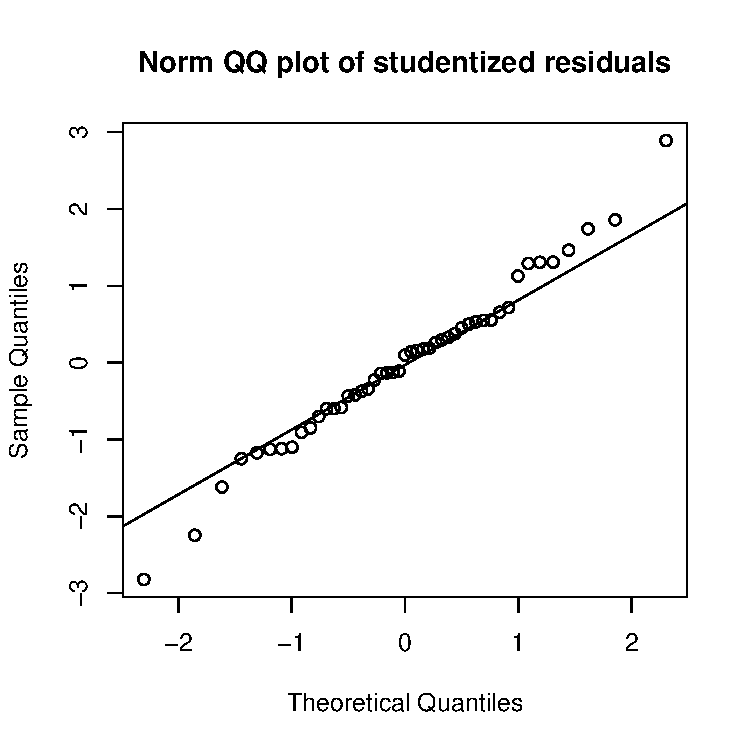
\includegraphics{part13-rstud-qq.pdf}
\end{center}

\end{document}


